\hypertarget{regions}{%
\section{Regions}\label{regions}}

\hypertarget{north-sea-countries}{%
\subsection{North Sea countries}\label{north-sea-countries}}

As per the definition provided by the European MSP Platform {[}NortND{]}
and the CPMR North Sea Commission {[}Memb15{]}, the North Sea region
consists of eight countries: Belgium, Denmark, France, Germany,
Netherlands, Norway, Sweden and United Kingdom.

\hypertarget{nuts-nomenclature-of-territorial-units-for-statistics}{%
\subsubsection{\texorpdfstring{\href{https://ec.europa.eu/eurostat/web/nuts/background}{NUTS
(Nomenclature of territorial units for
statistics)}}{NUTS (Nomenclature of territorial units for statistics)}}\label{nuts-nomenclature-of-territorial-units-for-statistics}}

\href{https://github.com/ENSYSTRA/short-term-forecasting/tree/master/jupyter-notebooks/NUTS.ipynb}{See
the Jupyter notebook}.

\hypertarget{bidding-zones}{%
\subsection{Bidding zones}\label{bidding-zones}}

\hypertarget{definition}{%
\subsubsection{Definition}\label{definition}}

According to {[}Bidd14{]}:

\begin{itemize}
\tightlist
\item
  The largest geographical area within which market participants are
  able to exchange energy without capacity allocation.
\item
  The majority of bidding zones in Europe are defined by national
  borders (e.g., France or the Netherlands).
\item
  Some are larger than national borders (e.g., Austria, Germany and
  Luxembourg or the Single Electricity Market for the island of Ireland)
\item
  Some are smaller zones within individual countries (e.g., Italy,
  Norway or Sweden).
\end{itemize}

\hypertarget{bidding-zones-in-the-north-sea-region}{%
\subsubsection{Bidding zones in the North Sea
region}\label{bidding-zones-in-the-north-sea-region}}

The bidding zones in the European electricity market are illustrated in
the map below {[}Tren17{]}.

\begin{figure}
\centering
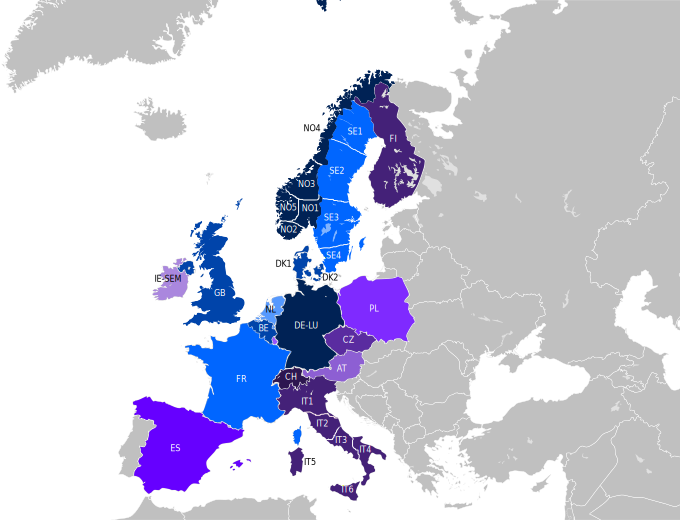
\includegraphics{images/market-map.png}
\caption{Bidding zones in the European electricity market. Source:
\href{http://raport.pse.pl/en/trends-and-market-context}{Polskie Sieci
Elektroenergetyczne} {[}Tren17{]}.}
\end{figure}

\begin{longtable}[]{@{}lll@{}}
\caption{Bidding zones in the North Sea region.}\tabularnewline
\toprule
\textbf{Country} & \textbf{Market(s)} & \textbf{Zone(s)}\tabularnewline
\midrule
\endfirsthead
\toprule
\textbf{Country} & \textbf{Market(s)} & \textbf{Zone(s)}\tabularnewline
\midrule
\endhead
Belgium (BE) & EPEX SPOT & BE\tabularnewline
Germany (DE / GE) & EPEX SPOT &
DE-AT-LU\protect\hyperlink{f4}{{[}f4{]}}\tabularnewline
Denmark (DK) & Nord Pool & DK1, DK2\tabularnewline
France (FR) & EPEX SPOT & FR\tabularnewline
Netherlands (NL) & EPEX SPOT & NL\tabularnewline
Norway (NO) & Nord Pool & NO1, NO2, NO3, NO4, NO5\tabularnewline
Sweden (SE / SW) & Nord Pool & SE1, SE2, SE3, SE4\tabularnewline
United Kingdom (UK) & EPEX SPOT, Nord Pool & GB,
I-SEM\protect\hyperlink{f4}{{[}f4{]}}\tabularnewline
\bottomrule
\end{longtable}

{[}f4{]} \emph{Austria (AT / AU); Luxembourg (LU); Great Britain (GB);
Irish single electricity market (I-SEM), which includes Republic of
Ireland (IE) and UK's Northern Ireland (NI).}

\hypertarget{transmission-system-operators-and-interconnections}{%
\subsubsection{Transmission system operators and
interconnections}\label{transmission-system-operators-and-interconnections}}

The power exchanges that operate in the North Sea region are EPEX SPOT
(Belgium, France, Germany, Netherlands, United Kingdom) and Nord Pool
(Denmark, Norway, Sweden, United Kingdom) {[}Over16{]}, {[}See ND{]},
{[}EPEXND{]}. The day-ahead market takes place generally as an hourly
auction 24 hours prior to dispatch {[}Over16{]}. The intra-day market
has continuous trading and will operate until two hours and up to five
minutes before dispatch {[}Over16{]}. The North Sea region consists of
multiple TSOs, cross-border interconnections and bidding zones, as
listed in the table below.

\begin{longtable}[]{@{}llll@{}}
\caption{TSOs and cross-border interconnections in the North Sea region.
Data: European Network of Transmission System Operators for Electricity
{[}ENTSND{]}, {[}RegiND{]}.}\tabularnewline
\toprule
\begin{minipage}[b]{0.07\columnwidth}\raggedright
Ctry.\protect\hyperlink{f5}{{[}f5{]}}\strut
\end{minipage} & \begin{minipage}[b]{0.37\columnwidth}\raggedright
TSOs\strut
\end{minipage} & \begin{minipage}[b]{0.22\columnwidth}\raggedright
Cross-border
interconnection\protect\hyperlink{f5}{{[}f5{]}},\protect\hyperlink{f6}{{[}f6{]}}\strut
\end{minipage} & \begin{minipage}[b]{0.22\columnwidth}\raggedright
Bidding
zones\protect\hyperlink{f5}{{[}f5{]}},\protect\hyperlink{f6}{{[}f6{]}}\strut
\end{minipage}\tabularnewline
\midrule
\endfirsthead
\toprule
\begin{minipage}[b]{0.07\columnwidth}\raggedright
Ctry.\protect\hyperlink{f5}{{[}f5{]}}\strut
\end{minipage} & \begin{minipage}[b]{0.37\columnwidth}\raggedright
TSOs\strut
\end{minipage} & \begin{minipage}[b]{0.22\columnwidth}\raggedright
Cross-border
interconnection\protect\hyperlink{f5}{{[}f5{]}},\protect\hyperlink{f6}{{[}f6{]}}\strut
\end{minipage} & \begin{minipage}[b]{0.22\columnwidth}\raggedright
Bidding
zones\protect\hyperlink{f5}{{[}f5{]}},\protect\hyperlink{f6}{{[}f6{]}}\strut
\end{minipage}\tabularnewline
\midrule
\endhead
\begin{minipage}[t]{0.07\columnwidth}\raggedright
BE\strut
\end{minipage} & \begin{minipage}[t]{0.37\columnwidth}\raggedright
Elia System Operator\strut
\end{minipage} & \begin{minipage}[t]{0.22\columnwidth}\raggedright
FR, LU, NL, UK\strut
\end{minipage} & \begin{minipage}[t]{0.22\columnwidth}\raggedright
BE\strut
\end{minipage}\tabularnewline
\begin{minipage}[t]{0.07\columnwidth}\raggedright
DK\strut
\end{minipage} & \begin{minipage}[t]{0.37\columnwidth}\raggedright
Energinet\strut
\end{minipage} & \begin{minipage}[t]{0.22\columnwidth}\raggedright
DE, NO, SE\strut
\end{minipage} & \begin{minipage}[t]{0.22\columnwidth}\raggedright
DK1, DK2\strut
\end{minipage}\tabularnewline
\begin{minipage}[t]{0.07\columnwidth}\raggedright
DE\strut
\end{minipage} & \begin{minipage}[t]{0.37\columnwidth}\raggedright
TransnetBW, TenneT TSO, Amprion, 50Hertz Transmission\strut
\end{minipage} & \begin{minipage}[t]{0.22\columnwidth}\raggedright
AT, CH, CZ, DK, FR, LU, NL, PL, SE\strut
\end{minipage} & \begin{minipage}[t]{0.22\columnwidth}\raggedright
CZ+DE+SK, DE-AT-LU, DE-LU\strut
\end{minipage}\tabularnewline
\begin{minipage}[t]{0.07\columnwidth}\raggedright
FR\strut
\end{minipage} & \begin{minipage}[t]{0.37\columnwidth}\raggedright
Réseau de Transport d'Electricité\strut
\end{minipage} & \begin{minipage}[t]{0.22\columnwidth}\raggedright
BE, CH, DE, ES, IT, UK\strut
\end{minipage} & \begin{minipage}[t]{0.22\columnwidth}\raggedright
FR\strut
\end{minipage}\tabularnewline
\begin{minipage}[t]{0.07\columnwidth}\raggedright
NL\strut
\end{minipage} & \begin{minipage}[t]{0.37\columnwidth}\raggedright
TenneT TSO\strut
\end{minipage} & \begin{minipage}[t]{0.22\columnwidth}\raggedright
BE, DE, NO, UK\strut
\end{minipage} & \begin{minipage}[t]{0.22\columnwidth}\raggedright
NL\strut
\end{minipage}\tabularnewline
\begin{minipage}[t]{0.07\columnwidth}\raggedright
NO\strut
\end{minipage} & \begin{minipage}[t]{0.37\columnwidth}\raggedright
Statnett\strut
\end{minipage} & \begin{minipage}[t]{0.22\columnwidth}\raggedright
DK, FI, NL, SE\strut
\end{minipage} & \begin{minipage}[t]{0.22\columnwidth}\raggedright
NO1, NO2, NO3, NO4, NO5\strut
\end{minipage}\tabularnewline
\begin{minipage}[t]{0.07\columnwidth}\raggedright
SE\strut
\end{minipage} & \begin{minipage}[t]{0.37\columnwidth}\raggedright
Svenska Kraftnät\strut
\end{minipage} & \begin{minipage}[t]{0.22\columnwidth}\raggedright
DK, FI, DE, LT, NO, PL\strut
\end{minipage} & \begin{minipage}[t]{0.22\columnwidth}\raggedright
SE1, SE2, SE3, SE4\strut
\end{minipage}\tabularnewline
\begin{minipage}[t]{0.07\columnwidth}\raggedright
UK\strut
\end{minipage} & \begin{minipage}[t]{0.37\columnwidth}\raggedright
National Grid Electricity Transmission, System Operator for Northern
Ireland, Scottish Hydro Electric Transmission, ScottishPower
Transmission\strut
\end{minipage} & \begin{minipage}[t]{0.22\columnwidth}\raggedright
BE, FR, IE, NL\strut
\end{minipage} & \begin{minipage}[t]{0.22\columnwidth}\raggedright
GB, IE (SEM)\strut
\end{minipage}\tabularnewline
\bottomrule
\end{longtable}

{[}f5{]} \emph{Ctry. - Country; AT - Austria; BE - Belgium; CH -
Switzerland; CZ - Czech Republic; DE - Germany; DK - Denmark; ES -
Spain; FI - Finland; FR - France; GB - Great Britain; IE - Ireland; IT -
Italy; LT - Lithuania; LU - Luxembourg; NL - Netherlands; NO - Norway;
PL - Poland; SE - Sweden; SK - Slovakia; UK - United Kingdom; SEM -
Single electricity market.}

{[}f6{]} \emph{These countries are not part of the North Sea region: AT,
CH, CZ, ES, FI, IE, IT, LT, LU, PL.}
